\documentclass[ams,openany,10pt,presentation,utf8]{mathbook}
\usepackage{kpfonts}
\usepackage{listings}
\usepackage{mathrsfs}
\definecolor{bleu}{cmyk}{0.59,0.11,0,0.59}
\definecolor{vert}{cmyk}{0.78,0,0.74,0.45}
\lstset{
	numbers=left, 
	numberstyle=\tiny, 
	stepnumber=1, 
	numbersep=3pt, 
	language=[LaTeX]TeX, 
	backgroundcolor=\color{bleu!20},
	frame=shadowbox,
	rulesepcolor=\color{bleu},
	rulecolor=\color{bleu},
	framexleftmargin=10pt,
	keywordstyle=\color{vert}\bfseries,
	basicstyle=\ttfamily,
    columns=flexible,
    keepspaces=true,
    upquote=true,
    commentstyle=\color{gray},
    morekeywords={redefineColor,dfrac,setlength,cellspacetoplimit, cellspacebottomlimit,firstline,text,intro,introauthor,chapter, itemclass,exostart,corrstart,AfficheCorriges,columnbreak,titlepic, nbcolindex,indexname,printindex,makeindex,activites, DefineNewBoxLikeRem,BreakCorr}
}
\usepackage{amssymb}
\usepackage{amsmath}
\usepackage{mathtools}
\usepackage{upgreek}
\usepackage{eucal}
\usepackage{verbatim}
%\usepackage{verse}
\usepackage{graphicx}
\usepackage{subfigure}
\usepackage{xcolor}
%\usepackage{makeidx}
\usepackage{multicol}
\usepackage{booktabs}
\usepackage{multirow}
\usepackage{float}
\usepackage{wrapfig}
\usepackage{caption}
\usepackage{siunitx}
\usepackage{array}
\usepackage{mdframed}
\usepackage{enumerate}
\usepackage{textcomp}


\graphicspath{
{chapters/chapter01/figures/}
{chapters/chapter02/figures/}
{chapters/chapter03/figures/}
{chapters/chapter04/figures/}
{chapters/chapter05/figures/}
{chapters/chapter06/figures/}
{chapters/chapter07/figures/}
{chapters/chapter08/figures/}
{chapters/chapter09/figures/}
{chapters/chapter10/figures/}
{chapters/chapter11/figures/}
{chapters/chapter12/figures/}
{chapters/chapter13/figures/}
{chapters/chapter14/figures/}
{chapters/chapter15/figures/}
{chapters/chapter16/figures/}
{chapters/chapter17/figures/}
{chapters/chapter18/figures/}
{chapters/chapter19/figures/}
{chapters/chapter20/figures/}
{chapters/chapter21/figures/}
{chapters/chapter22/figures/}
{chapters/chapter23/figures/}
{chapters/chapter24/figures/}
{chapters/chapter25/figures/}
{chapters/chapter26/figures/}
{chapters/chapter27/figures/}
{chapters/chapter28/figures/}
{chapters/chapter29/figures/}
{chapters/chapter30/figures/}
}

%\makeindex


%\includeonly{chapters/chapter02/sec1}

\begin{document}

\frontmatter

\title{高二物理竞赛教程}
\author{学而思物理}

\maketitle

{
\makeatletter
\sectiontitle@font
\tableofcontents
\makeatother
}


\mainmatter

%!TEX root = ../../Physics_XES_II.tex
\chapter{普通物理学概论}\label{1}

\intro{一些引入}

\section{范畴与方法论}\label{1-1}

self-contained: 数学知识有一定基础后不需要更多的补充

dependency-requalified: 
\[\text{力学}>\text{热学}>\text{电磁学}>\text{光学}>\text{近代物理}\]

picture-oriented: 由于数理基础不够而导致的有关物理原理背后的理论基础造成困难的现象, 我们企图用``物理图像''帮助读者理解其结果的自然性, 这样的章节用星号来标注, 读者不应当忽略其重要性, 应当在基础足够以后重新阅读相关章节.

读者也许知道, 矢量形式的\emph{牛顿力学}(Newtonian mechanics)理论, 和在其后发展出来的\emph{分析力学}(analytic mechanics)理论, 可以统称为\emph{经典力学}(classical mechanics)理论. 它们将是本书第I部分---力学的研究范围\footnote{分析力学仅做引入与概述.}. 而\emph{经典物理学}(classical physics)本书专指在二十世纪之前成熟的物理理论, 它还需要包括\emph{经典热力学}(classical thermodynamics)理论, 我们将在本书的第II部分---热学介绍; \emph{经典电磁学}(classical electrodynamics)理论, 我们将在本书的第III部分---电磁学介绍; 和\emph{几何光学}(geometric optics)与\emph{波动光学}(wave optics)理论, 我们将在本书的第IV部分---光学介绍.
%!TEX root = ../../Physics_XES_II.tex

\section{编排与客制化}\label{1-2}


%!TEX root = ../../Physics_XES_II.tex


\section{预备知识}\label{1-3}

\subsection{力学}\label{1-3-1}

\subsection{电磁学}\label{1-3-2}

\subsection{近代物理}\label{1-3-3}

\subsection{热学}\label{1-3-4}

\subsection{光学}\label{1-3-5}

\subsection{数学}\label{1-3-6}
%!TEX root = ../../Physics_XES_II.tex


\section*{总结}\label{1-1}




%!TEX root = ../../Physics_XES_II.tex

\section*{习题}\label{1-1}

\begin{exe}
some
\end{exe}

\begin{exe}
some
\end{exe}






\part{力学}

%!TEX root = ../../Physics_XES_II.tex
\chapterauthor{\sf 认识与描述物质的世界...}{}
%\chapterauthor{Second Author}{Second Author Affiliation}
\chapter{运动学}\label{2}

\emph{插图}



\section{时空与物质}\label{2-1}

物理学, 从刚开始成为实验性的科学的伽利略时期开始, 到近半个世纪年来理论物理学家对额外维度的探讨, 都给予了\emph{时空}(spacetime)最核心的地位. 牛顿的理论, 分析力学, 经典场论, 相对论这些理论最基本的图像都是时空与\emph{物质}(matter)的分立性. 时空是装备了一个能体现出物理物理意义的\emph{度量}(metric)的3+1维对象. 数学上有一套严格的说法, 把这种连续, 光滑的四维对象称为\emph{伪黎曼流形}(pseudo-Riemannian manifold). 而物质则是在每个时空点处的某种结构. 经典理论下, 这种结构不外乎用\emph{标量}(scalar), \emph{矢量}(vector)或是更高级的\emph{张量}(tensor)来描述. 最后, 这些量的变化就体现出了形形色色的\emph{运动}(motion). \emph{运动学}(kinematics)的主要任务就是描写物质的运动, 而对于物质运动背后体现出来的\emph{定律}(law), 我们仅做笼统的较浅的讨论, 更加深入地看, 不同物质运动符合的不同定律往往又需要因为时空的结构或相互作用的内禀属性而具有普遍的\emph{对称性}(symmetry), 对称性是``规律之规律'', 它对物理理论在何种程度上起到决定作用将是超出本书范围的更高层次的课题, 将伴随读者对物理学学习的生涯.

\subsection{时空观}\label{2-1-1}

牛顿力学理论体系基于\emph{伽利略时空观}(Galilean spacetime picture), 也就是\emph{绝对时空观}(absolute spacetime picture). 在这里空间是三维的平直空间. 设想一个人站在该空间的某个空间点, 他的胸前, 头顶和右手平举的三个方向就是相互垂直的方向. 如果以自己的臂长为标准长度, 他能够定义空间中每两个点之间的空间间隔. 事实上, 这个人能够以一种正确的方式为每个空间点定义一个坐标, 那么所有三维空间点的集合与任意两个点之间的距离为:

\[A(x,\,y,\,z)\in\mathbb{R}^3 \quad;\quad x,\,y,\,z\in\mathbb{R}\]
\[A(x_1,\,y_1,\,z_1)\;,\;B(x_2,\,y_2,\,z_2)\;:\;l^2=\overline{AB}^2=(x_1-x_2)^2+(y_1-y_2)^2+(z_1-z_2)^2\]

因为空间不同于时间, 我们为以上数字赋予特殊的物理含义, 也就是加上\emph{量纲}(dimension). 如果两点坐标为$(0,\,0,\,0)$和$(1,\,1,\,1)$, 那么$l= \si{\sqrt{3}m}$, 而不是$l=\sqrt{3}$. 其单位$\si{m}$一方面表示了这个物理量的属性, 另一方面指定了某个实际物理体系确定下来的固有长度大小. 现行的(2018年1月1日, 下文同)国际单位制对$\si{1m}$的定义如下\footnote{一方面, 它依赖于狭义相对论的正确性, 目前极少理论物理工作者会质疑它. 另一方面, 应该要先定义下文的$\si{1s}$, 再来定义$\si{1m}$.}:
\begin{verse}\sf\large
$\si{1m}$是光在$\si{\frac{1}{299792458}s}$内在真空中行进的距离.
\end{verse}


这就是我们的\emph{三维平直空间}(3-dimensional flat space). 注意空间点具有物理实际意义, 它可以脱离坐标系而单独存在. 事实上坐标系的原点可以建立在空间中的任意点处, 朝向也可以是任意方向, 两个空间点之间的距离$l$不会依赖于坐标系的选取, 但两个点的坐标会因坐标系不同而改变. 如果我们选取的坐标系总是下述使得两个相距很近的点之间的微元距离公式成立:
\[\ud l^2=\ud x^2+\ud y^2+\ud z^2\]


那么建立的坐标系就是一个\emph{笛卡尔坐标系}(Cartesian coordinate system), 即\emph{空间直角坐标系}(3D orthogonal coordinate system). 但是以空间直角坐标系为基础, 我们又经常建立\emph{球坐标}(spherical coordinate)和\emph{柱坐标}(cylindrical coordinate)系统. 通常取$x$轴为\emph{幅轴}(azimuth axis), 点在$x-y$平面上的投影与原点的连线相对$x$轴转过的角度为$\varphi$, 即\emph{幅角}(azimuth angle). 而$z$轴为\emph{极轴}(polar axis), 而点与原点连线与极轴的夹角$\theta$为\emph{极角}(polar angle). 天文观测用球坐标就很方便, 它是以描述的空间点到原点之间的距离$r$, 也称\emph{矢径}(radius), 和两个描述角位置的极角幅角来构成三个坐标$(r,\,\theta,\,\varphi)$的. 而理论物理里也常用到的柱坐标是以$(\rho,\,\varphi,\,z)$为描述空间点的坐标, $\rho$是空间点到$z$轴的距离.

\begin{wrapfigure}[16]{o}[-10pt]{7cm}
\vspace{-0.4cm}
\centering
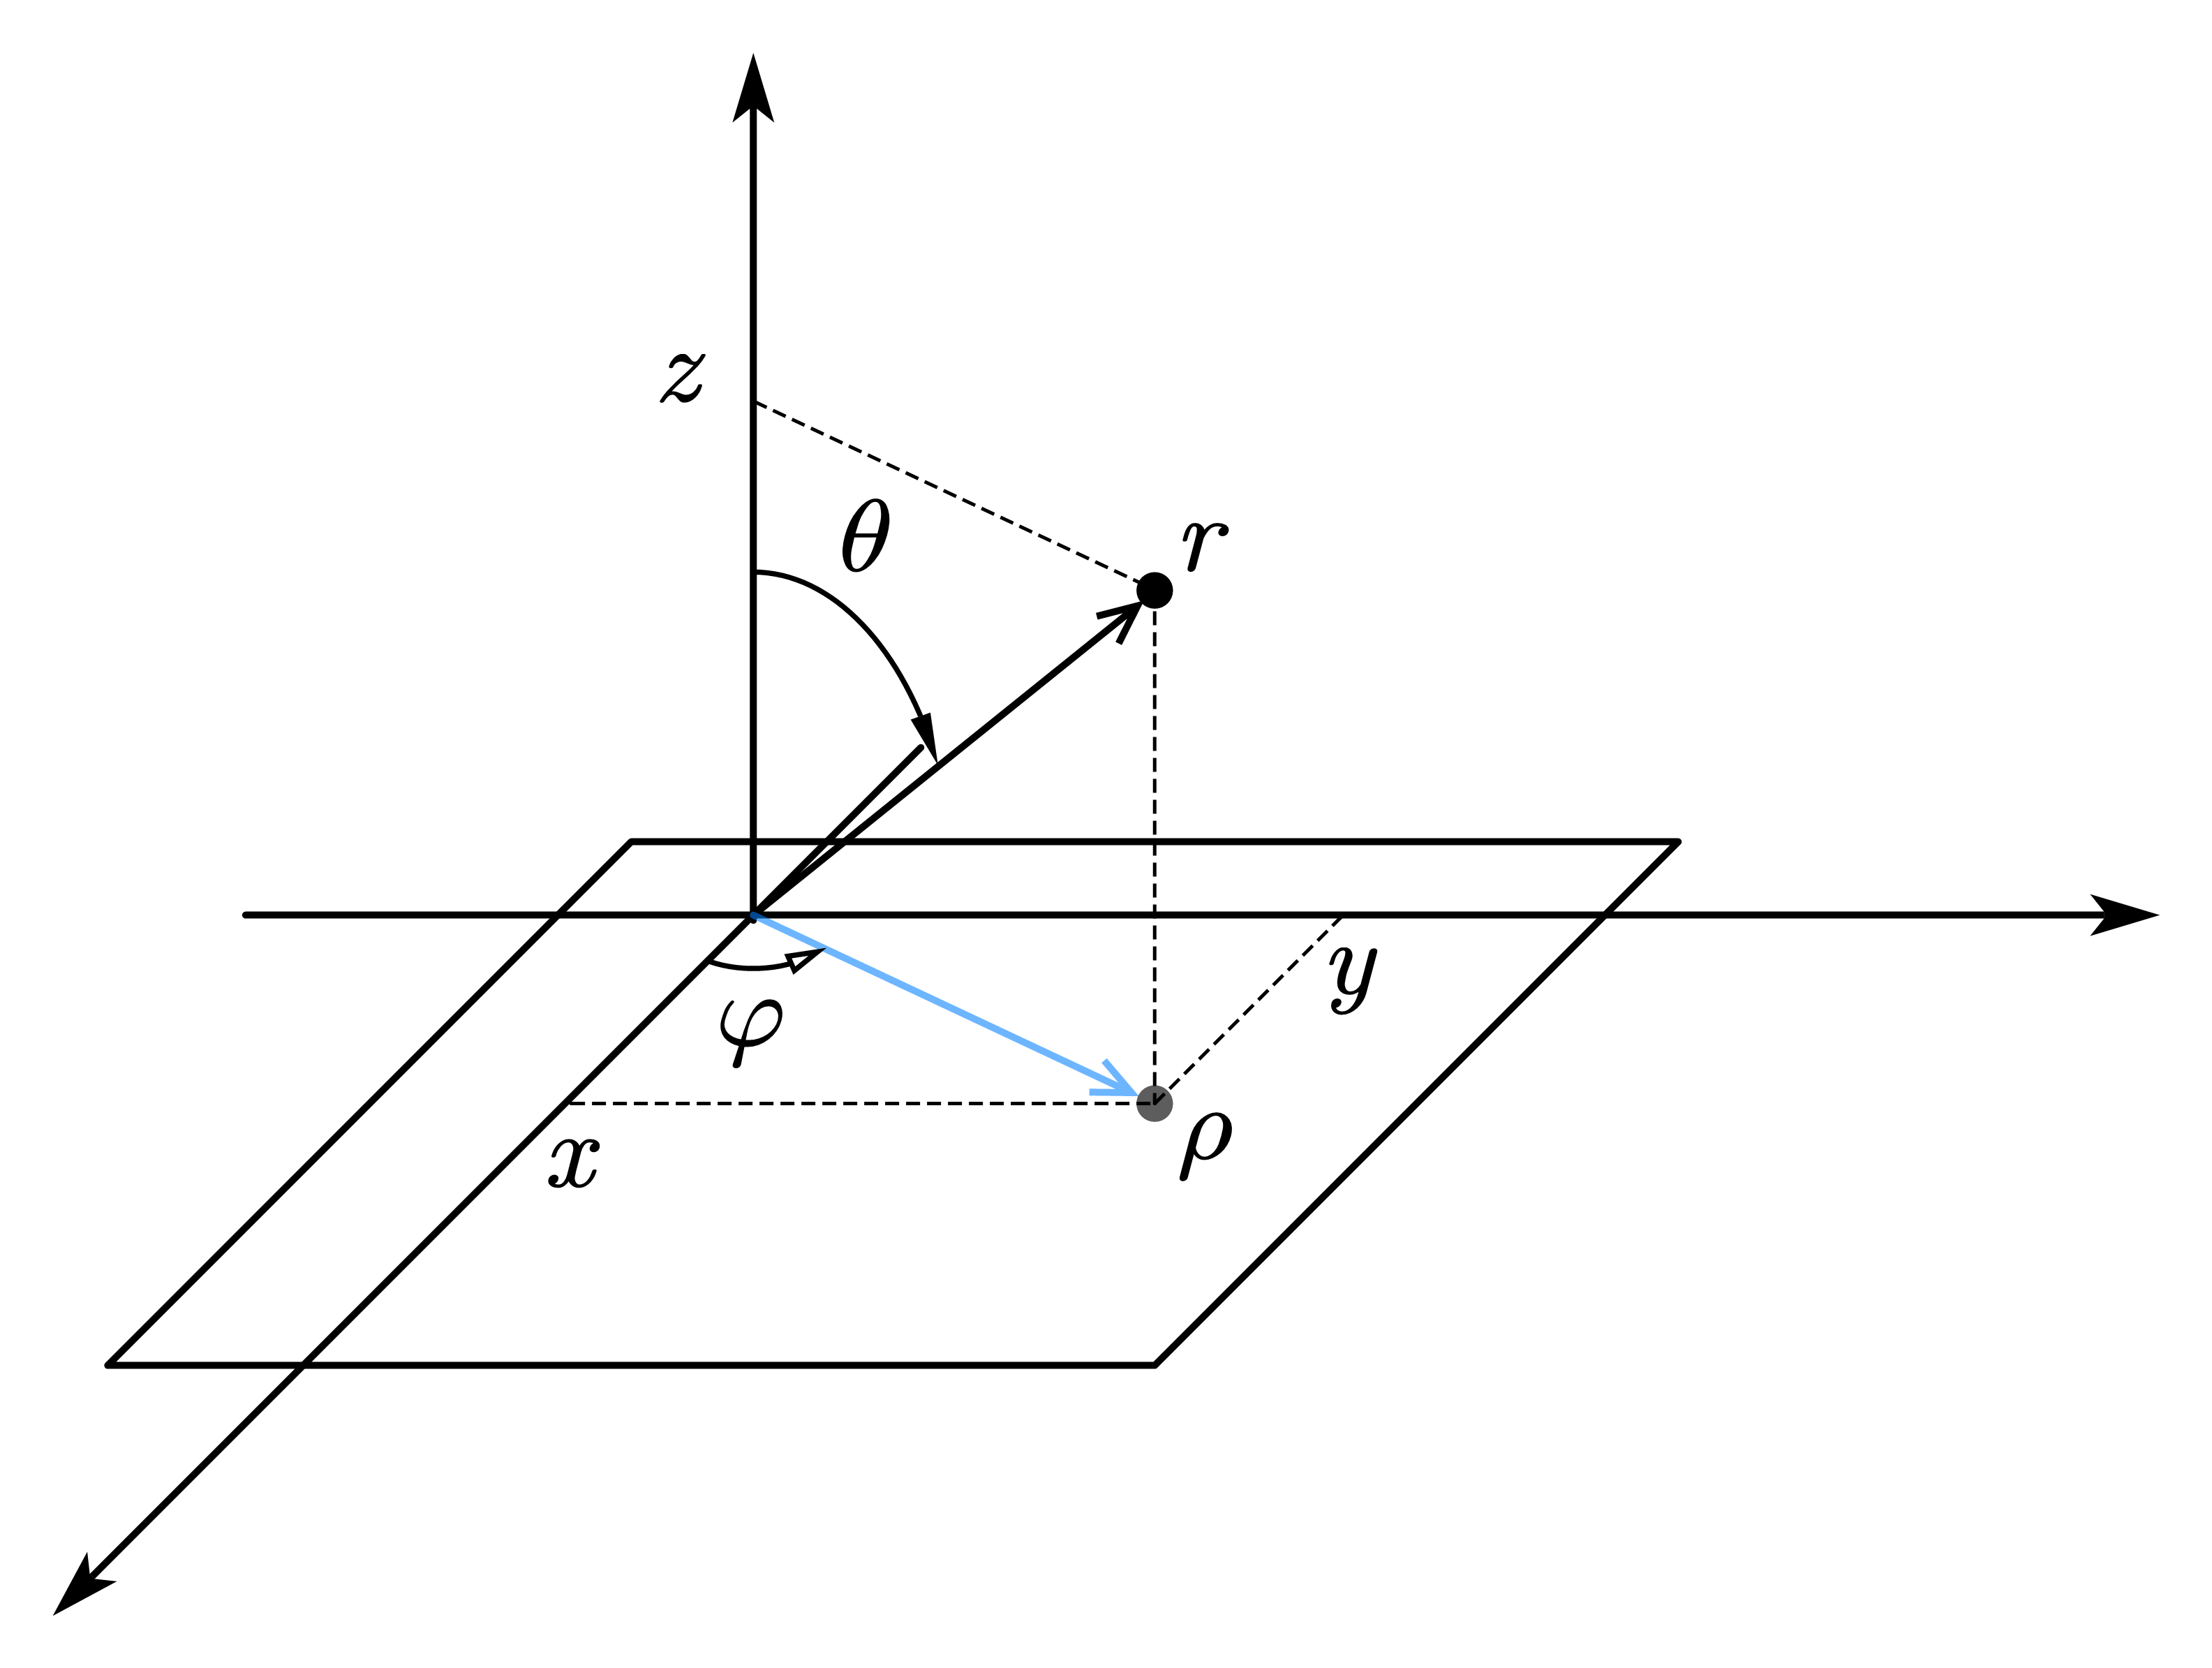
\includegraphics[width=7cm]{2.1.png}
\caption{三种坐标}
\end{wrapfigure}
之后经常会说到各种对称性, 在本系列教材中我们采取如下说法: \emph{球对称}(spherical symmetric)仅仅代表某个函数$f(r,\theta,\varphi)$与$\varphi$无关. 而\emph{柱对称}(cylindrical symmetric)代表的是$f(\rho,\,\varphi,\,z)$与$z$无关. 与$\varphi$和$\theta$都无关的$f(r,\,\theta,\,\varphi)=f(r,\,\forall\theta,\,\forall\varphi)$被称为\emph{各向同性}(isotropic). 最后\emph{中心对称}(centrosymmetric)是一个很弱的对称性, 它仅仅代表函数在\emph{中心反演}(space inversion)下的对称性:
\[f(x,\,y,\,z)=f(-x,\,-y,\,-z)\]

绝对时空观中的时间则是一种完全与空间独立的属性. 任意一个坐标点处都有时间轴, 而任意一个时刻都有一个三维空间切片. 事实上, 我们的时空是一个3+1维的结构, 合理地选取坐标后, 实际上可以把时空结构写成四维坐标:
\[A(x,\,y,\,z,\,t)\in\mathbb{R}^4 \quad;\quad x,\,y,\,z,\,t\in\mathbb{R}\]

时间是一个新的量纲, 其国际单位制对$1{\rm s}$的定义为:
\begin{verse}\sf\large
\si{1s}是$^{133}{\rm Cs}$原子基态的两个超精细能级之间跃迁所对应的辐射周期时长的$9192631770$倍.
\end{verse}

而对于任意两个时空点, 存在绝对的时间间隔, 也就是可以找到两个事件的绝对时间差:
\[\tau=|t_2-t_1|\]

但空间距离却具有相对性. 故我们要求在同一时刻的空间切片上定义空间的度量:
\[t_1=t_2:\quad l=\sqrt{(x_1-x_2)^2+(y_1-y_2)^2+(z_1-z_2)^2}\]

这种时空结构被叫做\emph{牛顿-嘉当几何}(Newton-Cartan geometry). 在牛顿-嘉当几何中书写的物理规律应当具有时空平移对称性, 空间旋转对称性和\emph{伽利略变换}(Galilean transformation)的对称性, 此后我们将进一步阐述. 时空平移是指将原来发生的物理过程随时空坐标进行如下改变:
\[\begin{cases}t \quad &\longrightarrow \quad t+\Delta t\\x \quad &\longrightarrow \quad x+\Delta x\\y \quad &\longrightarrow \quad y+\Delta y\\z \quad &\longrightarrow \quad z+\Delta z \end{cases} \]

空间旋转对称性的一种简单情况是绕$z$轴旋转$\theta$角:
\[\begin{cases}t \quad &\longrightarrow \quad t\\x \quad &\longrightarrow \quad x\cos\theta-y\sin\theta\\y \quad &\longrightarrow \quad y\cos\theta+x\sin\theta\\z \quad &\longrightarrow \quad z\end{cases} \]

伽利略变换是指不改变过程发生的时间, 但是对于不同时刻发生的事件的坐标进行重新标定, 从而使得两个坐标系之间恰好只差一个速度为$\bs{v}=(v_x,\,v_y,\,v_z)$的匀速直线运动:
\[\begin{cases}t \quad &\longrightarrow \quad t\\x \quad &\longrightarrow \quad x-v_x t\\y \quad &\longrightarrow \quad y-v_y t\\z \quad &\longrightarrow \quad z-v_z t \end{cases} \]




不同于绝对时空观中时间与空间成为相互独立的量纲的特点, 狭义相对论改变了对基本物理量的看法. 狭义相对论把时空看成为可以相互转化的不可分割的新的3+1维整体. 两个时空点之间无法定义绝对的时间间隔. 在\emph{相对论时空观}(relativistic spacetime picture)下, 时间和空间可以用同一把尺子去丈量: 这是由于光速的不变性:
\[c=299792458{\rm m/s}\]

而量出来的长度叫做\emph{时空间隔}(spacetime interval):
\[\ud s^2=c^2\ud t^2-\ud x^2-\ud y^2-\ud z^2\]

这赋予时空以截然不同的结构, 最关键的一点是, 时间顺序的绝对性被取消了, 相对论的有限速度因果律在这里取代了经典观点的时序因果律. 相对论理论我们将在此后章节展开介绍.

\subsection{物质观}\label{2-1-2}

时空是物理过程发生的舞台. 舞台上排演的剧目则是各式各样的\emph{物质}(matter)作为演员, 而根据其间的\emph{相互作用}(interaction)作为剧本而造就的\emph{可观测量}(observable)的变化. 任何物理理论, 描述物质的存在形式, 描述相互作用的形式当然以某些含\emph{物理量}(physical quantity)的公式作为数学载体. 但是, 不是所有物理量都一定是可观测量. 可观测量, 即可以测量的物理量, 读者也许会对这个概念感到陌生, 难道还有不可以测量的物理量吗? 当然有, 以下是两个例子:
\begin{enumerate}
	\item 研究交流电问题中, 将交流电流升格为相量(复数):
	\[i=I_0\cos(\omega t+\varphi) \quad \longrightarrow \quad \widetilde{I}=\frac{I_0}{\sqrt{2}}\ue^{\uj \left(\omega t+\varphi\right)}\]

	则虚部$\mathfrak{Im}\widetilde{I}$由于是人为引入的辅助性量而不是可观测量.

	\item 研究静电学问题中, 由于不一定选取无穷远为电势的零点, 故实际上一个静电学体系在某点产生的电势为:
	\[\varphi=\int\frac{\ud Q}{4\pi\varepsilon_0 r}+C\]

	所以同一个体系可能具有不同的$\varphi$, 即用$\varphi$去描述物理体系时存在冗余. 从而电势的绝对大小不是可观测量, 两个点电势的差值才是可观测量.

	\item ...

\end{enumerate}

对于一个物理理论来说, 基本定律中的物理量不一定是可观测量, 此时应当给出利用物理量计算可观测量的额外公式. 所幸在本书的大部分篇幅中, 各类物理量都是可以进行测量的. 故仅在遇到不可观测量时例外强调.

物理量可以分为两类: 第一类是时空坐标$\bs{r},\,t$, 它是物质运动在时空上的外化. 第二个类描述物质内禀的属性. 它取决于所引入的物质种类, 还取决于我们所关心问题的层次. 一般用\emph{标量}(scalar), \emph{矢量}(vector), 乃至\emph{张量}(tensor), \emph{旋量}(spinor)这样的数学工具来描述它. 举例, 电磁场物质在经典物理中用电场磁场来描述, 但在\emph{量子力学}(quantum mechanics,  QM)中这不够了, 需要用矢势和标势来描述才是完整的. 在更深的\emph{量子场论}(quantum field theory,  QFT)中甚至这也是不够的. 还需要量子化为光子才合适. 又比如, 电子参与的物理现象, 最简单的电子模型是质点模型, 其内禀的属性是质量, 动量与能量. 然而与电磁场的经典相互作用强度告诉我们还有一项内禀属性叫做电荷量. 近代人们惊奇地发现原来电子还固有磁矩, 与之相应的电子具有内禀的自旋. 最后狄拉克等人发展出\emph{量子电动力学}(quantum electrodynamics, QED), 统一地用一个四分量的旋量波函数就能完整地描述所有发现的电子内禀属性.


我们来看一些典型的关于物质的理论模型:

\subsubsection{质点模型}

不得不承认质点是牛顿力学的根基, 一切可观的结论的出发点. 质点所对应的事件集合为时空中的一条\emph{世界线}(world line). 每一个时间仅仅有可能只有一个事件发生. 实际上质点的运动用\emph{运动学方程}(kinematic equation)来描述:
\[\bs{r}=\bs{r}(t)=\left(x(t),\,y(t),\,z(t)\right)\]

而\emph{质量}(mass)是质点必要的内禀属性. 它将作为参数出现在下一节介绍的动力学方程中. 它反应物质受到同样大小的相互作用运动状态改变的难易程度. 国际单位制从1889年至2018年末对$1\rm kg$的定义如下:

\begin{verse}
1kg是保存在法国巴黎布勒特伊宫的国际计量局实验室的约47立方厘米立式铂铱合金小圆柱的质量. 当然, 出于实用考虑, 也是很多它的官方复制体的质量.
\end{verse}

这个定义今已经有一百多年了, 历史远长于其他六个国际基本单位. 但目前这一古老的定义方式已经被废除, 新的定义\footnote{一方面, 它依赖于狭义相对论和量子力学的正确性, 目前极少理论物理工作者会质疑它. 另一方面, 应该要先定义上文的1s和1m, 再来定义1kg.}为:

\begin{verse}
1kg被这样定义: 取普朗克常数的固定数值在单位$\rm kg\cdot m^2\cdot s^{-1}$下为$\rm 6.62607015\times 10^{-34}$.
\end{verse}

长度, 时间和质量为三大力学量纲, 量纲是物理量的属性, 物理量的表示方法为数值加单位, 每个量纲有自己独特的一套单位, 不同单位间差一个纯数的倍率. 在物理量的加减时量纲必须相同而且结果保持量纲不变. 但不同量纲物理量可以进行乘除而生成新的量纲. 除了简单的加减乘除的以上规则以外, 其他特殊函数必须只能作用在无量纲的纯数上. 这叫做\emph{量纲法则}(dimensional rules).




\subsection{世界观}\label{2-1-3}
%!TEX root = ../../Physics_XES_II.tex


\section{运动的描述}\label{2-2}

\subsection{质点的运动}\label{2-2-1}

\subsection{刚体的运动}\label{2-2-2}


%!TEX root = ../../Physics_XES_II.tex


\section{参考系变换}\label{2-3}

\subsection{质点运动的变换}\label{2-3-1}

\subsection{刚体运动的变换}\label{2-3-2}


%!TEX root = ../../Physics_XES_II.tex


\section{运动的牵连}\label{2-4}

\subsection{相交系}\label{2-4-1}

\subsection{接触系}\label{2-4-2}

\subsection{纯滚系}\label{2-4-3}
%!TEX root = ../../Physics_XES_II.tex


\section*{总结}\label{1-1}




%!TEX root = ../../Physics_XES_II.tex

\section*{习题}\label{1-1}

\begin{exe}
some
\end{exe}

\begin{exe}
some
\end{exe}





%!TEX root = ../../Physics_XES_II.tex
\chapterauthor{从牛顿力学的视角来看世界的规律...}{}
%\chapterauthor{Second Author}{Second Author Affiliation}
\chapter{动力学}\label{3}

章节概述引入

\section{牛顿定律}\label{3-1}

\subsection{牛顿第一定律}\label{3-1-1}

\subsection{牛顿第二定律}\label{3-1-2}

\subsection{牛顿第三定律}\label{3-1-3}

\subsection{质点系}\label{3-1-4}

\subsection{非惯性系}\label{3-1-5} 
%!TEX root = ../../Physics_XES_II.tex


\section{动量定律}\label{3-2}

\subsection{质点的动量}\label{3-2-1}

\subsection{质点系的动量}\label{3-2-2}


%!TEX root = ../../Physics_XES_II.tex


\section{角动量定律}\label{3-3}

\subsection{质点的角动量}\label{3-3-1}

\subsection{质点系的角动量}\label{3-3-2}


%!TEX root = ../../Physics_XES_II.tex


\section{能量定律}\label{3-4}

\subsection{质点的动能}\label{3-4-1}

\subsection{质点系的动能}\label{3-4-2}

\subsection{势能与其他能量}\label{3-4-3}
%!TEX root = ../../Physics_XES_II.tex


\section{动力学问题求解}\label{3-5}

\subsection{运动积分}\label{3-5-1}

\subsection{单坐标变量情况}\label{3-5-2}

\subsection{多坐标变量情况}\label{3-5-3}
%!TEX root = ../../Physics_XES_II.tex


\section{碰撞}\label{3-6}

\subsection{二质点弹性正碰}\label{3-6-1}

\subsection{若干拓广}\label{3-6-2}

\subsubsection{斜碰}\label{3-6-2-1}

\subsubsection{刚体碰撞}\label{3-6-2-2}

\subsubsection{带约束的碰撞}\label{3-6-2-3}

\subsubsection{多体碰撞}\label{3-6-2-3}

\subsection{*几个普遍定理}\label{3-6-3}
%!TEX root = ../../Physics_XES_II.tex


\section*{总结}\label{1-1}




%!TEX root = ../../Physics_XES_II.tex

\section*{习题}\label{1-1}

\begin{exe}
some
\end{exe}

\begin{exe}
some
\end{exe}





%!TEX root = ../../Physics_XES_II.tex
\chapterauthor{矢量力学的局限, 分析力学的预备...}{}
%\chapterauthor{Second Author}{Second Author Affiliation}
\chapter{静力学}\label{4}

章节概述引入

\section{约束}\label{4-1}

\subsection{约束的类型}\label{4-1-1}

\subsection{广义坐标}\label{4-1-2}

\subsection{主动力与被动力}\label{4-1-3}


%!TEX root = ../../Physics_XES_II.tex


\section{力系的简化}\label{4-2}

\subsection{静力学的公理体系}\label{4-2-1}

\subsection{力系简化原理}\label{4-2-2}

\subsubsection{若干结论}\label{4-2-2-1}

\subsubsection{平面力系简化的最终结果}\label{4-2-2-2}

\subsubsection{空间力系简化的最终结果}\label{4-2-2-3}
%!TEX root = ../../Physics_XES_II.tex


\section{平衡问题求解I}\label{4-3}

\subsection{平衡条件与平衡判据}\label{4-3-1}

\subsection{平衡问题的提法}\label{4-3-2}

\subsection{平衡问题的分类}\label{4-3-3}

\subsection{矢量力学的解决方案}\label{4-3-4}
%!TEX root = ../../Physics_XES_II.tex


\section{平衡问题求解II}\label{4-4}

\subsection{理想约束}\label{4-4-1}

\subsection{再论保守力}\label{4-4-2}

\subsection{分析力学的解决方案}\label{4-4-3}
%!TEX root = ../../Physics_XES_II.tex


\section{*分析力学基础}\label{4-5}

\subsection{力学的几何化}\label{4-5-1}

\subsection{拉格朗日方程}\label{4-5-2}

\subsection{再论冲击问题}\label{4-5-3}
%!TEX root = ../../Physics_XES_II.tex


\section{稳定性问题}\label{4-6}

\subsection{单自由度体系的平衡稳定性}\label{4-6-1}

\subsection{多自由度体系的平衡稳定性}\label{4-6-2}

\subsection{动力学稳定性}\label{4-6-3}
%!TEX root = ../../Physics_XES_II.tex


\section*{总结}\label{1-1}




%!TEX root = ../../Physics_XES_II.tex

\section*{习题}\label{1-1}

\begin{exe}
some
\end{exe}

\begin{exe}
some
\end{exe}





%!TEX root = ../../Physics_XES_II.tex
\chapter{简谐振动}\label{5}

章节概述引入

\section{谐振子}\label{5-1}

\subsection{简谐振动的定义}\label{5-1-1}

\subsection{简谐振动的运动学性质}\label{5-1-2}

\subsection{简谐振动的判定}\label{5-1-3}

\subsection{谐振子模型}\label{5-1-4}

%!TEX root = ../../Physics_XES_II.tex


\section{简谐振动的拓广}\label{5-2}

\subsection{阻尼振动}\label{5-2-1}

\subsection{受迫振动}\label{5-2-2}


%!TEX root = ../../Physics_XES_II.tex


\section{简单的多自由度小振动}\label{5-3}

\subsection{位形空间中的振动}\label{5-3-1}

\subsubsection{通过特征方程求解}\label{5-3-1-1}

\subsubsection{*通过坐标变换求解}\label{5-3-1-2}

\subsubsection{*通过对称性求解}\label{5-3-1-2}

\subsection{相空间中的振动}\label{5-3-2}


%!TEX root = ../../Physics_XES_II.tex


\section{*摄动理论}\label{5-4}

\subsection{线性情况}\label{5-4-1}

\subsection{非线性情况}\label{5-4-2}
%!TEX root = ../../Physics_XES_II.tex


\section{*可数无穷自由度情况}\label{5-5}

\subsection{格波}\label{5-5-1}
%!TEX root = ../../Physics_XES_II.tex


\section*{总结}\label{1-1}




%!TEX root = ../../Physics_XES_II.tex

\section*{习题}\label{1-1}

\begin{exe}
some
\end{exe}

\begin{exe}
some
\end{exe}





%!TEX root = ../../Physics_XES_II.tex
\chapter{万有引力}\label{6}

章节概述引入

\section{万有引力定律}\label{6-1}


%!TEX root = ../../Physics_XES_II.tex


\section{动量定律}\label{3-2}

\subsection{质点的动量}\label{3-2-1}

\subsection{质点系的动量}\label{3-2-2}


%!TEX root = ../../Physics_XES_II.tex


\section{开普勒问题}\label{6-3}

\subsection{轨道分类}\label{6-3-1}

\subsection{动力学量的计算}\label{6-3-2}

\subsection{摄动}\label{6-3-3}

\subsection{二体问题}\label{6-3-4}
%!TEX root = ../../Physics_XES_II.tex


\section{*潮汐}\label{6-4}

\subsection{引潮力}\label{6-4-1}

\subsection{若干应用}\label{6-4-2}

%!TEX root = ../../Physics_XES_II.tex


\section*{总结}\label{1-1}




%!TEX root = ../../Physics_XES_II.tex

\section*{习题}\label{1-1}

\begin{exe}
some
\end{exe}

\begin{exe}
some
\end{exe}





%!TEX root = ../../Physics_XES_II.tex
\chapterauthor{质点概念修改为质元, 建立新的理想模型: 讨论刚体的动力学...}{}
%\chapterauthor{Second Author}{Second Author Affiliation}
\chapter{刚体}\label{7}

章节概述引入

\section{刚体的物理描述}\label{7-1}

\subsection{刚体的运动}\label{7-1-1}

\subsection{质量几何}\label{7-1-2}
%!TEX root = ../../Physics_XES_II.tex


\section{动量定律}\label{3-2}

\subsection{质点的动量}\label{3-2-1}

\subsection{质点系的动量}\label{3-2-2}


%!TEX root = ../../Physics_XES_II.tex


\section{*刚体的空间运动}\label{7-3}

\subsection{惯量张量}\label{7-3-1}

\subsection{欧拉运动学方程}\label{7-3-2}

\subsection{欧拉动力学方程}\label{7-3-3}
%!TEX root = ../../Physics_XES_II.tex


\section*{总结}\label{1-1}




%!TEX root = ../../Physics_XES_II.tex

\section*{习题}\label{1-1}

\begin{exe}
some
\end{exe}

\begin{exe}
some
\end{exe}





%!TEX root = ../../Physics_XES_II.tex
\chapterauthor{当连续介质的内相互作用力正比于其形变...}{}
%\chapterauthor{Second Author}{Second Author Affiliation}
\chapter{*弹性体}\label{8}

章节概述引入

\section{弹性体的物理描述}\label{8-1}

\subsection{应变}\label{8-1-1}

\subsection{应力}\label{8-1-2}

%!TEX root = ../../Physics_XES_II.tex


\section{动量定律}\label{3-2}

\subsection{质点的动量}\label{3-2-1}

\subsection{质点系的动量}\label{3-2-2}


%!TEX root = ../../Physics_XES_II.tex


\section{角动量定律}\label{3-3}

\subsection{质点的角动量}\label{3-3-1}

\subsection{质点系的角动量}\label{3-3-2}


%!TEX root = ../../Physics_XES_II.tex


\section*{总结}\label{1-1}




%!TEX root = ../../Physics_XES_II.tex

\section*{习题}\label{1-1}

\begin{exe}
some
\end{exe}

\begin{exe}
some
\end{exe}





%!TEX root = ../../Physics_XES_II.tex
\chapterauthor{当连续介质不再具有恢复形变的能力...}{学而思物理竞赛团队}
%\chapterauthor{Second Author}{Second Author Affiliation}
\chapter{流体}\label{9}

章节概述引入

\section{流体的物理描述}\label{9-1}

\subsection{连续性方程}\label{9-1-1}

\subsection{应变率}\label{9-1-2}

\subsection{压强与黏滞}\label{9-1-3}
%!TEX root = ../../Physics_XES_II.tex


\section{动量定律}\label{3-2}

\subsection{质点的动量}\label{3-2-1}

\subsection{质点系的动量}\label{3-2-2}


%!TEX root = ../../Physics_XES_II.tex


\section{黏滞流体动力学}\label{9-3}

\subsection{牛顿黏滞定律}\label{9-3-1}

\subsection{*两个常用定律}\label{9-3-2}

\subsection{*纳维-斯托克斯方程}\label{9-3-3}
%!TEX root = ../../Physics_XES_II.tex


\section{*流体中的波}\label{9-4}

\subsection{浅水波}\label{9-4-1}

\subsection{深水波}\label{9-4-2}

\subsection{表面波}\label{9-4-3}
%!TEX root = ../../Physics_XES_II.tex


\section{动力学问题求解}\label{3-5}

\subsection{运动积分}\label{3-5-1}

\subsection{单坐标变量情况}\label{3-5-2}

\subsection{多坐标变量情况}\label{3-5-3}
%!TEX root = ../../Physics_XES_II.tex


\section*{总结}\label{1-1}




%!TEX root = ../../Physics_XES_II.tex

\section*{习题}\label{1-1}

\begin{exe}
some
\end{exe}

\begin{exe}
some
\end{exe}






\part{热学}


%!TEX root = ../../Physics_XES_II.tex
\chapterauthor{电荷的阴阳激荡产生了整个电磁学学科, 当电荷静止时就会产生静电场...}{}
%\chapterauthor{Second Author}{Second Author Affiliation}
\chapter{静电学}\label{10}

章节概述引入

\section{电荷与电场}\label{10-1}

\subsection{电荷}\label{10-1-1}

\subsection{库仑定律}\label{10-1-2}

\subsection{电场}\label{10-1-3}
%!TEX root = ../../Physics_XES_II.tex


\section{两个定律与电势}\label{10-2}

\subsection{电场通量定律}\label{10-2-1}

\subsection{电势与电场环量定律}\label{10-2-2}

\subsection{*高速运动电荷的电场}\label{10-2-3}
%!TEX root = ../../Physics_XES_II.tex


\section{角动量定律}\label{3-3}

\subsection{质点的角动量}\label{3-3-1}

\subsection{质点系的角动量}\label{3-3-2}


%!TEX root = ../../Physics_XES_II.tex


\section{常见气体模型}\label{10-4}

\subsection{混合理想气体}\label{10-4-1}

\subsection{范德瓦尔斯气体}\label{10-4-2}

\subsection{重力场中的大气}\label{10-4-3}

\subsection{再论流体的定常流动}\label{10-4-4}

\subsubsection{欧拉方程}\label{10-4-4-1}

\subsubsection{伯努利方程}\label{10-4-4-2}

\subsubsection{*传导形式与守恒形式}\label{10-4-4-3}
%!TEX root = ../../Physics_XES_II.tex


\section*{总结}\label{1-1}




%!TEX root = ../../Physics_XES_II.tex

\section*{习题}\label{1-1}

\begin{exe}
some
\end{exe}

\begin{exe}
some
\end{exe}





%!TEX root = ../../Physics_XES_II.tex
\chapterauthor{作者}{学而思物理竞赛团队}
%\chapterauthor{Second Author}{Second Author Affiliation}
\chapter{章}\label{1}

章节概述引入

\section{节}\label{1-1}

\subsection{小节}\label{1-1-1}

\subsubsection{小小节}\label{1-1-1-1}


%!TEX root = ../../Physics_XES_II.tex


\section{动量定律}\label{3-2}

\subsection{质点的动量}\label{3-2-1}

\subsection{质点系的动量}\label{3-2-2}


%!TEX root = ../../Physics_XES_II.tex


\section{热力学第二定律}\label{11-3}

\subsection{熵增原理}\label{11-3-1}

\subsection{两种等效表述}\label{11-3-2}

\subsection{再论卡诺定理}\label{11-3-3}

\subsection{克劳修斯不等式}\label{11-3-4}
%!TEX root = ../../Physics_XES_II.tex


\section{能量定律}\label{3-4}

\subsection{质点的动能}\label{3-4-1}

\subsection{质点系的动能}\label{3-4-2}

\subsection{势能与其他能量}\label{3-4-3}
%!TEX root = ../../Physics_XES_II.tex


\section{动力学问题求解}\label{3-5}

\subsection{运动积分}\label{3-5-1}

\subsection{单坐标变量情况}\label{3-5-2}

\subsection{多坐标变量情况}\label{3-5-3}
%!TEX root = ../../Physics_XES_II.tex


\section*{总结}\label{1-1}




%!TEX root = ../../Physics_XES_II.tex

\section*{习题}\label{1-1}

\begin{exe}
some
\end{exe}

\begin{exe}
some
\end{exe}





%!TEX root = ../../Physics_XES_II.tex
\chapterauthor{面对复杂多体问题, 我们唯象地描述背后的物理...}{}
%\chapterauthor{Second Author}{Second Author Affiliation}
\chapter{固体与液体性质}\label{12}

章节概述引入

\section{固体晶格论}\label{12-1}

\subsection{经典晶格论}\label{12-1-1}

\subsection{*量子晶格论}\label{12-1-2}

%!TEX root = ../../Physics_XES_II.tex


\section{*固体电子论}\label{12-2}

\subsection{线性输运现象}\label{12-2-1}

\subsection{热电耦合现象}\label{12-2-2}

\subsection{德鲁特模型}\label{12-2-3}

\subsection{能带模型与半导体}\label{12-2-4}
%!TEX root = ../../Physics_XES_II.tex


\section{角动量定律}\label{3-3}

\subsection{质点的角动量}\label{3-3-1}

\subsection{质点系的角动量}\label{3-3-2}


%!TEX root = ../../Physics_XES_II.tex


\section{液体的表面性质}\label{12-4}

\subsection{表面与界面的热学性质}\label{12-4-1}

\subsection{附加压强}\label{12-4-2}

\subsection{接触角}\label{12-4-3}
%!TEX root = ../../Physics_XES_II.tex


\section{动力学问题求解}\label{3-5}

\subsection{运动积分}\label{3-5-1}

\subsection{单坐标变量情况}\label{3-5-2}

\subsection{多坐标变量情况}\label{3-5-3}
%!TEX root = ../../Physics_XES_II.tex


\section*{总结}\label{1-1}




%!TEX root = ../../Physics_XES_II.tex

\section*{习题}\label{1-1}

\begin{exe}
some
\end{exe}

\begin{exe}
some
\end{exe}





%!TEX root = ../../Physics_XES_II.tex
\chapterauthor{作者}{学而思物理竞赛团队}
%\chapterauthor{Second Author}{Second Author Affiliation}
\chapter{章}\label{1}

章节概述引入

\section{节}\label{1-1}

\subsection{小节}\label{1-1-1}

\subsubsection{小小节}\label{1-1-1-1}


%!TEX root = ../../Physics_XES_II.tex


\section{相变}\label{13-2}

\subsection{一级相变特性}\label{13-2-1}

\subsection{气液相变}\label{13-2-2}

\subsection{*溶解与沉积}\label{13-2-3}

\subsection{*顺磁-铁磁相变}\label{13-2-4}

\subsection{*二级相变特性}\label{13-2-4}
%!TEX root = ../../Physics_XES_II.tex


\section{角动量定律}\label{3-3}

\subsection{质点的角动量}\label{3-3-1}

\subsection{质点系的角动量}\label{3-3-2}


%!TEX root = ../../Physics_XES_II.tex


\section*{总结}\label{1-1}




%!TEX root = ../../Physics_XES_II.tex

\section*{习题}\label{1-1}

\begin{exe}
some
\end{exe}

\begin{exe}
some
\end{exe}





%!TEX root = ../../Physics_XES_II.tex
\chapterauthor{作者}{学而思物理竞赛团队}
%\chapterauthor{Second Author}{Second Author Affiliation}
\chapter{章}\label{1}

章节概述引入

\section{节}\label{1-1}

\subsection{小节}\label{1-1-1}

\subsubsection{小小节}\label{1-1-1-1}


%!TEX root = ../../Physics_XES_II.tex


\section{动量定律}\label{3-2}

\subsection{质点的动量}\label{3-2-1}

\subsection{质点系的动量}\label{3-2-2}


%!TEX root = ../../Physics_XES_II.tex


\section{麦克斯韦分布律}\label{14-3}

\subsection{麦克斯韦速度分布律}\label{14-3-1}

\subsection{压强与泻流}\label{14-3-2}

\subsection{*输运系数的计算}\label{14-3-3}

%!TEX root = ../../Physics_XES_II.tex


\section{麦克斯韦-玻尔兹曼统计}\label{14-4}

\subsection{分布律}\label{14-4-1}

\subsection{压强与内能的计算}\label{14-4-2}

\subsection{功, 热, 熵的微观解释}\label{14-4-3}
%!TEX root = ../../Physics_XES_II.tex


\section{*其他物理统计模型}\label{14-5}

\subsection{玻色-爱因斯坦统计}\label{14-5-1}

\subsection{费米-狄拉克统计}\label{14-5-2}

\subsection{涨落与关联}\label{14-5-3}
%!TEX root = ../../Physics_XES_II.tex


\section*{总结}\label{1-1}




%!TEX root = ../../Physics_XES_II.tex

\section*{习题}\label{1-1}

\begin{exe}
some
\end{exe}

\begin{exe}
some
\end{exe}





\part{电磁学}

%!TEX root = ../../Physics_XES_II.tex
\chapterauthor{作者}{学而思物理竞赛团队}
%\chapterauthor{Second Author}{Second Author Affiliation}
\chapter{章}\label{1}

章节概述引入

\section{节}\label{1-1}

\subsection{小节}\label{1-1-1}

\subsubsection{小小节}\label{1-1-1-1}


%!TEX root = ../../Physics_XES_II.tex


\section{动量定律}\label{3-2}

\subsection{质点的动量}\label{3-2-1}

\subsection{质点系的动量}\label{3-2-2}


%!TEX root = ../../Physics_XES_II.tex


\section{角动量定律}\label{3-3}

\subsection{质点的角动量}\label{3-3-1}

\subsection{质点系的角动量}\label{3-3-2}


%!TEX root = ../../Physics_XES_II.tex


\section{能量定律}\label{3-4}

\subsection{质点的动能}\label{3-4-1}

\subsection{质点系的动能}\label{3-4-2}

\subsection{势能与其他能量}\label{3-4-3}
%!TEX root = ../../Physics_XES_II.tex


\section*{总结}\label{1-1}




%!TEX root = ../../Physics_XES_II.tex

\section*{习题}\label{1-1}

\begin{exe}
some
\end{exe}

\begin{exe}
some
\end{exe}





%!TEX root = ../../Physics_XES_II.tex
\chapterauthor{作者}{学而思物理竞赛团队}
%\chapterauthor{Second Author}{Second Author Affiliation}
\chapter{章}\label{1}

章节概述引入

\section{节}\label{1-1}

\subsection{小节}\label{1-1-1}

\subsubsection{小小节}\label{1-1-1-1}


%!TEX root = ../../Physics_XES_II.tex


\section{动量定律}\label{3-2}

\subsection{质点的动量}\label{3-2-1}

\subsection{质点系的动量}\label{3-2-2}


%!TEX root = ../../Physics_XES_II.tex


\section{电介质}\label{16-3}

\subsection{微观角度理解极化}\label{16-3-1}

\subsubsection{位移极化}\label{16-3-1-1}

\subsubsection{取向极化}\label{16-3-1-2}

\subsection{宏观角度理解极化}\label{16-3-2}

\subsubsection{电位移}\label{16-3-2-1}

\subsubsection{简单体系的静电平衡}\label{16-3-2-2}

\subsubsection{介质中的静电平衡}\label{16-3-2-3}

\subsection{宏观与微观的联系}\label{16-3-3}
%!TEX root = ../../Physics_XES_II.tex


\section{能量定律}\label{3-4}

\subsection{质点的动能}\label{3-4-1}

\subsection{质点系的动能}\label{3-4-2}

\subsection{势能与其他能量}\label{3-4-3}
%!TEX root = ../../Physics_XES_II.tex


\section*{总结}\label{1-1}




%!TEX root = ../../Physics_XES_II.tex

\section*{习题}\label{1-1}

\begin{exe}
some
\end{exe}

\begin{exe}
some
\end{exe}





%!TEX root = ../../Physics_XES_II.tex
\chapterauthor{作者}{学而思物理竞赛团队}
%\chapterauthor{Second Author}{Second Author Affiliation}
\chapter{章}\label{1}

章节概述引入

\section{节}\label{1-1}

\subsection{小节}\label{1-1-1}

\subsubsection{小小节}\label{1-1-1-1}


%!TEX root = ../../Physics_XES_II.tex


\section{动量定律}\label{3-2}

\subsection{质点的动量}\label{3-2-1}

\subsection{质点系的动量}\label{3-2-2}


%!TEX root = ../../Physics_XES_II.tex


\section{电路分析基础}\label{17-3}

\subsection{电路的整体性质}\label{17-3-1}

\subsection{电路求解套路}\label{17-3-2}

\subsubsection{支路电流法}\label{17-3-2-1}

\subsubsection{节点电势法}\label{17-3-2-2}

\subsubsection{网孔电流法}\label{17-3-2-3}
%!TEX root = ../../Physics_XES_II.tex


\section{电路分析方法}\label{17-4}

\subsection{叠加原理}\label{17-4-1}

\subsection{戴维南-诺尔顿原理}\label{17-4-2}

\subsection{*特勒根原理}\label{17-4-3}

\subsection{*互易原理}\label{17-4-4}
%!TEX root = ../../Physics_XES_II.tex


\section{动力学问题求解}\label{3-5}

\subsection{运动积分}\label{3-5-1}

\subsection{单坐标变量情况}\label{3-5-2}

\subsection{多坐标变量情况}\label{3-5-3}
%!TEX root = ../../Physics_XES_II.tex


\section{碰撞}\label{3-6}

\subsection{二质点弹性正碰}\label{3-6-1}

\subsection{若干拓广}\label{3-6-2}

\subsubsection{斜碰}\label{3-6-2-1}

\subsubsection{刚体碰撞}\label{3-6-2-2}

\subsubsection{带约束的碰撞}\label{3-6-2-3}

\subsubsection{多体碰撞}\label{3-6-2-3}

\subsection{*几个普遍定理}\label{3-6-3}
%!TEX root = ../../Physics_XES_II.tex


\section*{总结}\label{1-1}




%!TEX root = ../../Physics_XES_II.tex

\section*{习题}\label{1-1}

\begin{exe}
some
\end{exe}

\begin{exe}
some
\end{exe}





%!TEX root = ../../Physics_XES_II.tex
\chapterauthor{作者}{学而思物理竞赛团队}
%\chapterauthor{Second Author}{Second Author Affiliation}
\chapter{章}\label{1}

章节概述引入

\section{节}\label{1-1}

\subsection{小节}\label{1-1-1}

\subsubsection{小小节}\label{1-1-1-1}


%!TEX root = ../../Physics_XES_II.tex


\section{两个定律与电势}\label{18-2}

\subsection{磁场环量定律}\label{18-2-1}

\subsection{矢势与磁场通量定律}\label{18-2-2}

%!TEX root = ../../Physics_XES_II.tex


\section{角动量定律}\label{3-3}

\subsection{质点的角动量}\label{3-3-1}

\subsection{质点系的角动量}\label{3-3-2}


%!TEX root = ../../Physics_XES_II.tex


\section{磁介质与磁能}\label{18-4}

\subsection{微观角度理解磁化}\label{18-4-1}

\subsubsection{顺磁性}\label{18-4-1-1}

\subsubsection{抗磁性}\label{18-4-1-2}

\subsubsection{铁磁性}\label{18-4-1-3}

\subsection{宏观角度理解磁化}\label{18-4-2}

\subsubsection{磁场强度}\label{18-4-2-1}

\subsubsection{磁路定律}\label{18-4-2-2}

\subsubsection{电感}\label{18-4-2-3}

\subsection{磁场能量}\label{18-4-3}
%!TEX root = ../../Physics_XES_II.tex


\section*{总结}\label{1-1}




%!TEX root = ../../Physics_XES_II.tex

\section*{习题}\label{1-1}

\begin{exe}
some
\end{exe}

\begin{exe}
some
\end{exe}





%!TEX root = ../../Physics_XES_II.tex
\chapter{电磁感应}\label{19}

章节概述引入

\section{磁生电}\label{19-1}

\subsection{法拉第电磁感应定律}\label{19-1-1}

\subsection{动生电动势}\label{19-1-2}

\subsection{感生电动势}\label{19-1-3}

%!TEX root = ../../Physics_XES_II.tex


\section{电磁感应与电路}\label{19-2}

\subsection{例: 平行导轨}\label{19-2-1}

\subsection{发电机与电动机}\label{19-2-2}

\subsection{*涡电流}\label{19-2-3}

%!TEX root = ../../Physics_XES_II.tex


\section{角动量定律}\label{3-3}

\subsection{质点的角动量}\label{3-3-1}

\subsection{质点系的角动量}\label{3-3-2}


%!TEX root = ../../Physics_XES_II.tex


\section{能量定律}\label{3-4}

\subsection{质点的动能}\label{3-4-1}

\subsection{质点系的动能}\label{3-4-2}

\subsection{势能与其他能量}\label{3-4-3}
%!TEX root = ../../Physics_XES_II.tex


\section*{总结}\label{1-1}




%!TEX root = ../../Physics_XES_II.tex

\section*{习题}\label{1-1}

\begin{exe}
some
\end{exe}

\begin{exe}
some
\end{exe}





%!TEX root = ../../Physics_XES_II.tex
\chapterauthor{集齐电磁理论拼图的最后一块, 经典电磁学发展到了其最高峰...}{}
%\chapterauthor{Second Author}{Second Author Affiliation}
\chapter{麦克斯韦方程组}\label{20}

章节概述引入

\section{电生磁}\label{20-1}

\subsection{位移电流}\label{20-1-1}

\subsection{麦克斯韦方程组}\label{20-1-2}


%!TEX root = ../../Physics_XES_II.tex


\section{电磁波解}\label{20-2}

\subsection{真空中的电磁波}\label{20-2-1}

\subsection{介质中的电磁波}\label{20-2-2}

\subsection{电磁场的能量与动量}\label{20-2-3}
%!TEX root = ../../Physics_XES_II.tex


\section{角动量定律}\label{3-3}

\subsection{质点的角动量}\label{3-3-1}

\subsection{质点系的角动量}\label{3-3-2}


%!TEX root = ../../Physics_XES_II.tex


\section{能量定律}\label{3-4}

\subsection{质点的动能}\label{3-4-1}

\subsection{质点系的动能}\label{3-4-2}

\subsection{势能与其他能量}\label{3-4-3}
%!TEX root = ../../Physics_XES_II.tex


\section*{总结}\label{1-1}




%!TEX root = ../../Physics_XES_II.tex

\section*{习题}\label{1-1}

\begin{exe}
some
\end{exe}

\begin{exe}
some
\end{exe}





%!TEX root = ../../Physics_XES_II.tex
\chapterauthor{作者}{学而思物理竞赛团队}
%\chapterauthor{Second Author}{Second Author Affiliation}
\chapter{章}\label{1}

章节概述引入

\section{节}\label{1-1}

\subsection{小节}\label{1-1-1}

\subsubsection{小小节}\label{1-1-1-1}


%!TEX root = ../../Physics_XES_II.tex


\section{动量定律}\label{3-2}

\subsection{质点的动量}\label{3-2-1}

\subsection{质点系的动量}\label{3-2-2}


%!TEX root = ../../Physics_XES_II.tex


\section{交流电路解法}\label{21-3}

\subsection{复数解法}\label{21-3-1}

\subsection{相量图解}\label{21-3-2}

\subsection{功率分析}\label{21-3-3}
%!TEX root = ../../Physics_XES_II.tex


\section{能量定律}\label{3-4}

\subsection{质点的动能}\label{3-4-1}

\subsection{质点系的动能}\label{3-4-2}

\subsection{势能与其他能量}\label{3-4-3}
%!TEX root = ../../Physics_XES_II.tex


\section*{总结}\label{1-1}




%!TEX root = ../../Physics_XES_II.tex

\section*{习题}\label{1-1}

\begin{exe}
some
\end{exe}

\begin{exe}
some
\end{exe}






\part{光学}

%!TEX root = ../../Physics_XES_II.tex
\chapterauthor{作者}{学而思物理竞赛团队}
%\chapterauthor{Second Author}{Second Author Affiliation}
\chapter{章}\label{1}

章节概述引入

\section{节}\label{1-1}

\subsection{小节}\label{1-1-1}

\subsubsection{小小节}\label{1-1-1-1}


%!TEX root = ../../Physics_XES_II.tex


\section{动量定律}\label{3-2}

\subsection{质点的动量}\label{3-2-1}

\subsection{质点系的动量}\label{3-2-2}


%!TEX root = ../../Physics_XES_II.tex


\section{角动量定律}\label{3-3}

\subsection{质点的角动量}\label{3-3-1}

\subsection{质点系的角动量}\label{3-3-2}


%!TEX root = ../../Physics_XES_II.tex


\section{从费马到费曼}\label{22-4}

\subsection{费马原理}\label{22-4-1}

\subsection{惠更斯-菲涅尔原理}\label{22-4-2}

\subsection{*基尔霍夫衍射积分公式}\label{22-4-3}

\subsection{*费曼路径积分理论}\label{22-4-4}

\subsection{结论}\label{22-4-5}
%!TEX root = ../../Physics_XES_II.tex


\section*{总结}\label{1-1}




%!TEX root = ../../Physics_XES_II.tex

\section*{习题}\label{1-1}

\begin{exe}
some
\end{exe}

\begin{exe}
some
\end{exe}





%!TEX root = ../../Physics_XES_II.tex
\chapterauthor{作者}{学而思物理竞赛团队}
%\chapterauthor{Second Author}{Second Author Affiliation}
\chapter{章}\label{1}

章节概述引入

\section{节}\label{1-1}

\subsection{小节}\label{1-1-1}

\subsubsection{小小节}\label{1-1-1-1}


%!TEX root = ../../Physics_XES_II.tex


\section{动量定律}\label{3-2}

\subsection{质点的动量}\label{3-2-1}

\subsection{质点系的动量}\label{3-2-2}


%!TEX root = ../../Physics_XES_II.tex


\section{动量定律}\label{3-2}

\subsection{质点的动量}\label{3-2-1}

\subsection{质点系的动量}\label{3-2-2}


%!TEX root = ../../Physics_XES_II.tex


\section*{总结}\label{1-1}




%!TEX root = ../../Physics_XES_II.tex

\section*{习题}\label{1-1}

\begin{exe}
some
\end{exe}

\begin{exe}
some
\end{exe}





%!TEX root = ../../Physics_XES_II.tex
\chapterauthor{作者}{学而思物理竞赛团队}
%\chapterauthor{Second Author}{Second Author Affiliation}
\chapter{章}\label{1}

章节概述引入

\section{节}\label{1-1}

\subsection{小节}\label{1-1-1}

\subsubsection{小小节}\label{1-1-1-1}


%!TEX root = ../../Physics_XES_II.tex


\section{动量定律}\label{3-2}

\subsection{质点的动量}\label{3-2-1}

\subsection{质点系的动量}\label{3-2-2}


%!TEX root = ../../Physics_XES_II.tex


\section{助视仪器}\label{24-3}

\subsection{人眼与眼睛}\label{24-3-1}

\subsection{光学显微镜}\label{24-3-2}

\subsection{光学望远镜}\label{24-3-3}
%!TEX root = ../../Physics_XES_II.tex


\section{观像仪器}\label{24-4}

\subsection{数字相机}\label{24-4-1}

\subsection{透视仪}\label{24-4-2}

\subsection{电镜}\label{24-4-3}
%!TEX root = ../../Physics_XES_II.tex


\section*{总结}\label{1-1}




%!TEX root = ../../Physics_XES_II.tex

\section*{习题}\label{1-1}

\begin{exe}
some
\end{exe}

\begin{exe}
some
\end{exe}





%!TEX root = ../../Physics_XES_II.tex
\chapter{光的干涉}\label{25}

章节概述引入

\section{干涉引论}\label{25-1}

\subsection{波前函数}\label{25-1-1}

\subsection{傍轴近似与远场近似}\label{25-1-2}

\subsection{相干度}\label{25-1-3}

%!TEX root = ../../Physics_XES_II.tex


\section{动量定律}\label{3-2}

\subsection{质点的动量}\label{3-2-1}

\subsection{质点系的动量}\label{3-2-2}


%!TEX root = ../../Physics_XES_II.tex


\section{角动量定律}\label{3-3}

\subsection{质点的角动量}\label{3-3-1}

\subsection{质点系的角动量}\label{3-3-2}


%!TEX root = ../../Physics_XES_II.tex


\section{能量定律}\label{3-4}

\subsection{质点的动能}\label{3-4-1}

\subsection{质点系的动能}\label{3-4-2}

\subsection{势能与其他能量}\label{3-4-3}
%!TEX root = ../../Physics_XES_II.tex


\section*{总结}\label{1-1}




%!TEX root = ../../Physics_XES_II.tex

\section*{习题}\label{1-1}

\begin{exe}
some
\end{exe}

\begin{exe}
some
\end{exe}





%!TEX root = ../../Physics_XES_II.tex
\chapter{光的衍射}\label{26}

章节概述引入

\section{多光束干涉}\label{26-1}

\subsection{分振幅的多光束干涉}\label{26-1-1}

\subsection{分波面的多光束干涉}\label{26-1-2}

\subsection{X射线晶体衍射}\label{26-1-3}

%!TEX root = ../../Physics_XES_II.tex


\section{动量定律}\label{3-2}

\subsection{质点的动量}\label{3-2-1}

\subsection{质点系的动量}\label{3-2-2}


%!TEX root = ../../Physics_XES_II.tex


\section{角动量定律}\label{3-3}

\subsection{质点的角动量}\label{3-3-1}

\subsection{质点系的角动量}\label{3-3-2}


%!TEX root = ../../Physics_XES_II.tex


\section*{总结}\label{1-1}




%!TEX root = ../../Physics_XES_II.tex

\section*{习题}\label{1-1}

\begin{exe}
some
\end{exe}

\begin{exe}
some
\end{exe}





%!TEX root = ../../Physics_XES_II.tex
\chapterauthor{历史螺旋上升, 智慧历久弥新, 真理越辩越明...}{}
%\chapterauthor{Second Author}{Second Author Affiliation}
\chapter{物理光学}\label{27}

章节概述引入

\section{牛顿定律}\label{27-1}

\subsection{牛顿第一定律}\label{27-1-1}

\subsection{牛顿第二定律}\label{27-1-2}

\subsection{牛顿第三定律}\label{27-1-3}

\subsection{质点系}\label{27-1-4}

\subsection{非惯性系}\label{27-1-5}
%!TEX root = ../../Physics_XES_II.tex


\section{动量定律}\label{3-2}

\subsection{质点的动量}\label{3-2-1}

\subsection{质点系的动量}\label{3-2-2}


%!TEX root = ../../Physics_XES_II.tex


\section{角动量定律}\label{3-3}

\subsection{质点的角动量}\label{3-3-1}

\subsection{质点系的角动量}\label{3-3-2}


%!TEX root = ../../Physics_XES_II.tex


\section{能量定律}\label{3-4}

\subsection{质点的动能}\label{3-4-1}

\subsection{质点系的动能}\label{3-4-2}

\subsection{势能与其他能量}\label{3-4-3}
%!TEX root = ../../Physics_XES_II.tex


\section*{总结}\label{1-1}




%!TEX root = ../../Physics_XES_II.tex

\section*{习题}\label{1-1}

\begin{exe}
some
\end{exe}

\begin{exe}
some
\end{exe}





\part{近代物理}

%!TEX root = ../../Physics_XES_II.tex
\chapter{相对论}\label{28}

章节概述引入

\section{时空与运动}\label{28-1}

\subsection{相对论时空观}\label{28-1-1}

\subsection{尺缩, 钟慢, 同时相对性}\label{28-1-2}

\subsection{洛伦兹变换}\label{28-1-3}

\subsection{速度变换}\label{28-1-4}

\subsection{转盘佯谬}\label{28-1-5}
%!TEX root = ../../Physics_XES_II.tex


\section{动量定律}\label{3-2}

\subsection{质点的动量}\label{3-2-1}

\subsection{质点系的动量}\label{3-2-2}


%!TEX root = ../../Physics_XES_II.tex


\section{连续体}\label{28-3}

\subsection{四维波矢变换}\label{28-3-1}

\subsection{四维电流变换}\label{28-3-2}

\subsection{电磁场变换}\label{28-3-3}

%!TEX root = ../../Physics_XES_II.tex


\section{广义相对论简介}\label{28-4}

\subsection{度规与测地线}\label{28-4-1}

\subsection{弯曲的时空}\label{28-4-2}

\subsection{施瓦西黑洞}\label{28-4-3}
%!TEX root = ../../Physics_XES_II.tex


\section*{总结}\label{1-1}




%!TEX root = ../../Physics_XES_II.tex

\section*{习题}\label{1-1}

\begin{exe}
some
\end{exe}

\begin{exe}
some
\end{exe}





%!TEX root = ../../Physics_XES_II.tex
\chapterauthor{颠覆经典图像, 重建量子对应, 将上下而求索...}{}
%\chapterauthor{Second Author}{Second Author Affiliation}
\chapter{量子论}\label{29}

章节概述引入

\section{光的量子性}\label{29-1}

\subsection{黑体辐射}\label{29-1-1}

\subsection{光电效应}\label{29-1-2}

\subsection{康普顿效应}\label{29-1-3}

\subsection{*引力与光}\label{29-1-4}

%!TEX root = ../../Physics_XES_II.tex


\section{动量定律}\label{3-2}

\subsection{质点的动量}\label{3-2-1}

\subsection{质点系的动量}\label{3-2-2}


%!TEX root = ../../Physics_XES_II.tex


\section{*量子力学初步}\label{29-3}

\subsection{运动-波函数}\label{29-3-1}

\subsection{相互作用-算符}\label{29-3-2}

\subsection{波的动力学}\label{29-3-3}

\subsection{全同粒子与福克空间}\label{29-3-4}
%!TEX root = ../../Physics_XES_II.tex


\section*{总结}\label{1-1}




%!TEX root = ../../Physics_XES_II.tex

\section*{习题}\label{1-1}

\begin{exe}
some
\end{exe}

\begin{exe}
some
\end{exe}





%!TEX root = ../../Physics_XES_II.tex
\chapter{尺度物理学}\label{30}

章节概述引入

\section{基本粒子与相互作用}\label{30-1}

\subsection{标准模型}\label{30-1-1}

\subsection{相互作用过程}\label{30-1-2}

\subsection{守恒律}\label{30-1-3}

\subsection{*超越标准模型}\label{30-1-4}

%!TEX root = ../../Physics_XES_II.tex


\section{核物理}\label{30-2}

\subsection{核模型}\label{30-2-1}

\subsection{核反应}\label{30-2-2}

\subsection{核应用}\label{31-2-3}
%!TEX root = ../../Physics_XES_II.tex


\section{角动量定律}\label{3-3}

\subsection{质点的角动量}\label{3-3-1}

\subsection{质点系的角动量}\label{3-3-2}


%!TEX root = ../../Physics_XES_II.tex


\section{*介观物理}\label{30-4}

\subsection{声子模型}\label{30-4-1}

\subsection{电子气}\label{30-4-2}

\subsection{能带论}\label{30-4-3}

\subsection{强关联电子体系}\label{30-4-4}
%!TEX root = ../../Physics_XES_II.tex


\section{动力学问题求解}\label{3-5}

\subsection{运动积分}\label{3-5-1}

\subsection{单坐标变量情况}\label{3-5-2}

\subsection{多坐标变量情况}\label{3-5-3}
%!TEX root = ../../Physics_XES_II.tex


\section*{总结}\label{1-1}




%!TEX root = ../../Physics_XES_II.tex

\section*{习题}\label{1-1}

\begin{exe}
some
\end{exe}

\begin{exe}
some
\end{exe}






%\bibliographystyle{plain}
%\bibliography{bibtex_example}


%\printindex

\end{document}
